\chapter{はじめに} \label{intro}
\pagenumbering{arabic}  %% ページ番号をアラビア数字に変更

高等学校での物理学の授業では、実験が重要である。
Holubova~\cite{holubova_2019}は「実験室での作業は理論的な概念を検証する最も重要な方法であり、生徒は実験を通してどのような現象が起きるかを確認することができる」と述べている。

しかし実際は、生徒全員が実験を経験しているわけではない。林らは、2014年に大学生を対象に物理実験の経験を調査した~\cite{2015KJ00010038066}。これによると、力学分野で最も基本的な「運動の法則」に関する実験経験は60\%であった。また、斜方投射の基本的な問題である「モンキーハンティング~(図~\ref{monkey_hunting})」に関する実験は10\%に満たない。
理由としては、実験用の装置の準備や測定が難しいことや、実験を行うのに時間を要することが考えられる。

\begin{figure}[htb]
\noindent\rule{\linewidth}{0.4pt}
\begin{quote}
小球を、位置 $(0, 0)$ から初速 $v_0$、 仰角 $\theta$ で発射したところ、位置 $(l, h)$ から自由落下してくる物体に衝突した。 $\tan \theta$ の満たすべき条件を求めよ。ただし、重力加速度の大きさを $g$ とする。
\end{quote}
\centering
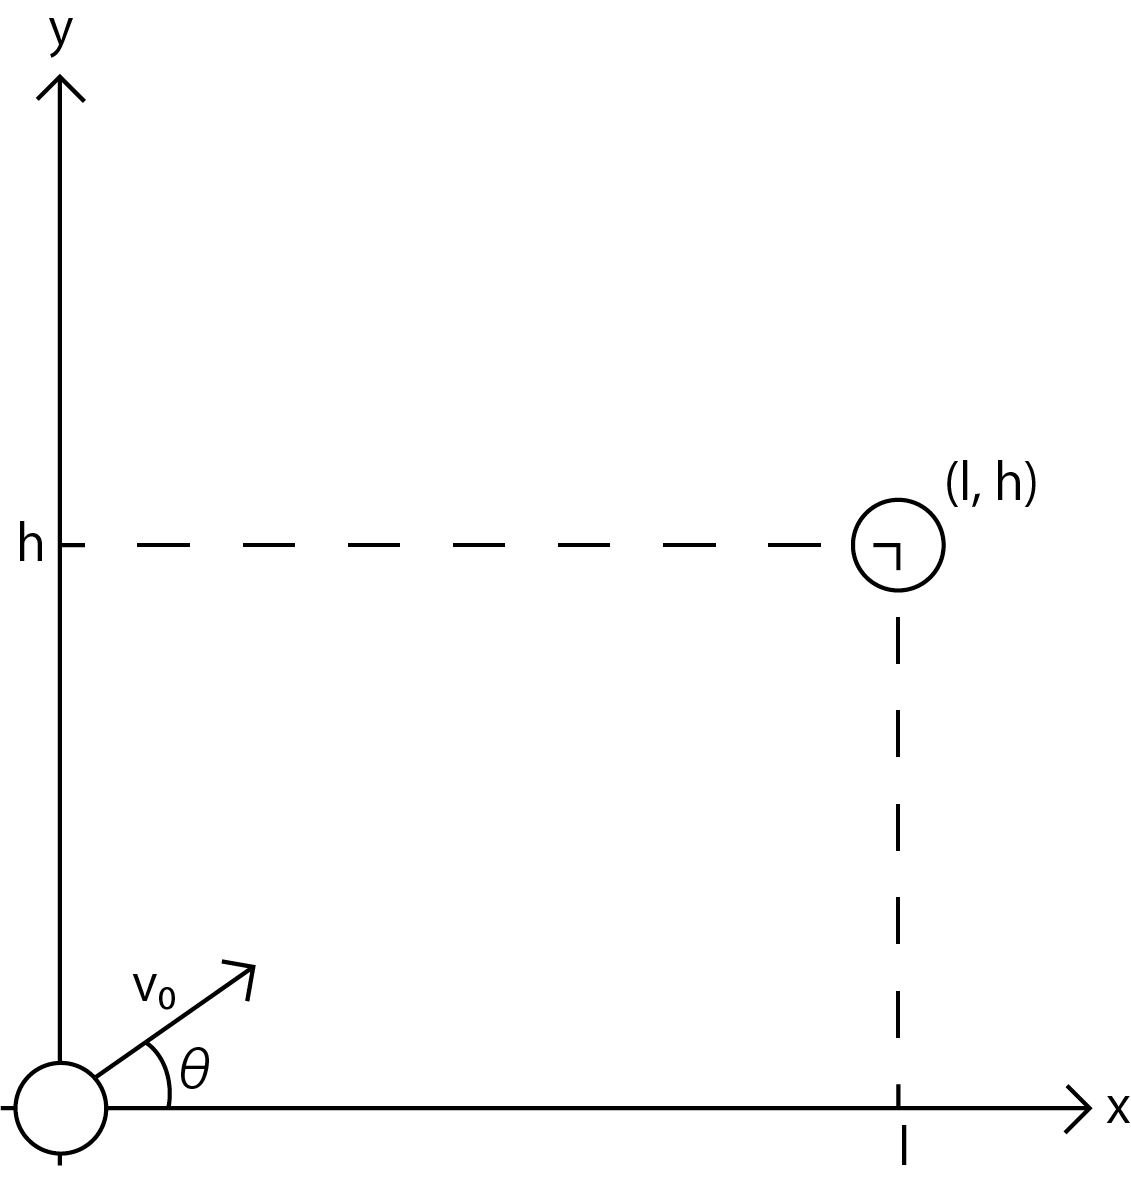
\includegraphics[width=0.3\linewidth]{work/monkey_hunting.png}
\caption{モンキーハンティング} \label{monkey_hunting}
\end{figure}

そこで実験の代替として近年利用されているのが、物理実験のシミュレータである。シミュレータを用いることで、実験と同様の学習効果を得ることができる。Ajredini~\cite{ajredini_real_2014} は、既存の物理実験シミュレータである PhET~\cite{perkins_phet_2006} を用いる授業と実際に実験を行う授業を実施し、テストを行った。その結果、シミュレーションによって得られる知識と実際の実験によって得られる知識の間には有意な差はないと結論づけた。

% TODO: この2つの段落、議論が既存のシミュレータ -> 一般的な物理の学習 -> 既存のシミュレータと行ったり来たりしていますね。
% 1. 一般的な物理の学習と既存のシミュレータの間には隔たりがある
% 2. 物理の学習ではこんなことをする
% 3. シミュレータではこれができない
% のような流れで書くのはいかがでしょうか。

しかし既存のシミュレータでは、学習者は可視化されている運動とその背景に存在する数式の間の関係を理解することは容易ではない。
学習者が理論を学習するとき、物理法則やそれを前提とした物体の運動を方程式を通して学習する。
図~\ref{symbol_based}は実際に生徒が扱うシチュエーションの例
%TODO: \cite{}
である。
学習者は、まず教科書等で物理法則を方程式として学習する。現実の運動を表す際は、学習した物理法則を基に方程式で表現する。
一方既存のシミュレータでは、教育者が物理法則から現象を数式で記述し、シミュレーションに変換しており、学習者は可視化されている運動とその背景に存在する数式の間の関係を理解することは容易ではない。既存のシミュレータである PhET では、図~\ref{numeral_based}のように速度や質量、位置のような物理量を数値でしか確認できず、描画されている物理系がどのような方程式によって表現されているのかわからない。そのため、学習者はシミュレーションを見ることで現実の物理現象を確認することができるが、それと物理法則との関係性は授業などで学ぶのみである。\\\\
% TODO: 具体的な弊害
% TODO: 他のシミュレータも列挙


\begin{figure}[htb]
\noindent\rule{\linewidth}{0.4pt}

ボールを $x$ 軸方向の初速 $v_{0x}$、$y$ 軸方向の初速 $v_{0y}$ で投げる。このとき、ボールがどのような軌道を描くか考える。ただし、重力加速度の大きさを g とする。投げる時刻を $t=0$ とする。等加速度運動の公式より、時刻 $t$ における位置 $x, y$ は次のように表される:
\begin{align}
  x &= v_{0x}t \label{斜方投射x}\\
  y &= v_{0y}t - \dfrac{1}{2}gt^2 \label{斜方投射y}
\end{align}
(\ref{斜方投射x}) より、$t = \dfrac{x}{v_{0x}}$ 。(\ref{斜方投射y}) に代入して、$y = \dfrac{v_{0y}}{v_{0x}}x - \dfrac{1}{2}\dfrac{g}{v_{0x}^2}x^2 = - \left(x - \dfrac{v_{0y}}{2 v_{0x}}\right)^{2} + \dfrac{v_{0y}^{2}}{4 v_{0x}^{2}}$ よって、頂点を $\left(\dfrac{v_{0y}}{2 v_{0x}} ,\dfrac{v_{0y}^{2}}{4 v_{0x}^{2}}\right)$ とする放物線を描く。

% \small{\textbf{(問題)} 静止している質量 $m$ の物体に大きさ $F$ の力をかけ続ける。$t$ 秒後の速さを求めよ。}

% \small{\textbf{(解答)} 物体の加速度を $a$ とする。運動方程式より $ma~=~F$ $\therefore~a~=~\dfrac{F}{m}$ 。等加速度運動の公式より $v~=~at~=~\dfrac{F}{m}t$\\
% 答え: $\dfrac{F}{m}t$}

\caption{学習者が方程式で物理現象を表現する例} \label{symbol_based}
\end{figure}

\begin{figure}[htb]
\centering
\includegraphics*[width=0.9\linewidth]{figure/PhET_example.png}
\caption{PhET のシミュレーション例} \label{numeral_based}
\end{figure}

現実の物理現象と物理法則との関係性は、学習者自身が物理法則から現象を数式で記述し、その振る舞いを観測することでよりよく理解できると思われる。誤った定義をすると想定外の動作をし、そこから物理法則や方程式の細部に対する考察を学習者自身が行うことも期待できる。

そこで本研究では、学習者に物理系を定義させるシミュレータ \simnamealt~(\simname) を提案する。学習者は \simname で系内の物体をそのパラメータとともに定義し、その物体の運動を表す方程式を立式する。シミュレーションを実行すると、定義した物理系に基づいて数値計算がなされ、物体の運動が可視化される。これにより、現実の物理現象と物理法則の間の対応を学習者自らの経験を通して理解することができると考えられる。この際学習者は、\simname に実装された動作例を参考にすることで、定義した物理系と現実の運動を比較することができたり、次元の異なる物理量の和が存在する不正な方程式を立式すると警告されるなど、正しい物理系を作成するための補助を受ける。

本論文の構成は以下の通りである。
第\ref{background}章で、斜方投射を通して既存のシミュレータでの表現について説明する。
第\ref{idea}章で、\simname の構成を説明する。
第\ref{implementation}章で、\simname の実現方法について説明する。
第\ref{related}章で、既存のシミュレータを用いた実例について紹介する。
第\ref{conclusion}章で、まとめと今後の展望について述べる。
